\chapter{The jSCAPE System}

The jSCAPE system is designed for two distinct groups of users: students and teachers/lecturers. This separation of roles lead to the development of the main application for students, and an administrator tool for teachers/lecturers.

\begin{figure}[H]
\centering
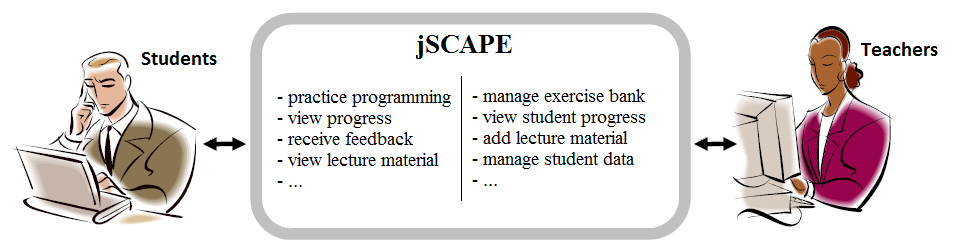
\includegraphics[width=\textwidth,height=\textheight,keepaspectratio]{jscape_use_case}
\caption{Use case diagram of the jSCAPE system.}
\label{fig:jscape_use_case}
\end{figure}

Figure \ref{fig:jscape_use_case} shows some of the main capabilities of the jSCAPE system. Students can practice their understanding of programming concepts by answering exercises provided by the lecturers, and receive feedback while doing so. In addition, students can track their progress by viewing various graphs and charts of their performance on particular exercise categories. Finally, students can access lecture notes and website links provided by the teacher. \newline

Teachers can manage the exercise bank, whether it be adding exercises manually or automatically generating new ones based on templates. They can keep track of their students' progress and thereby identify any difficulties particular students are having. Finally, teachers are responsible for adding lecture material, website links and creating student profiles to store in the database.\newline

In the rest of this chapter we take a closer look at the current available features of jSCAPE.\newline

At the time of writing this report, we would like to note that the screen shots of the application do not represent the final version of jSCAPE, in particular, the graphics and logos haven't been finalized.

\section{Student view}

\subsection{Login screen}
\begin{figure}[H]
\centering
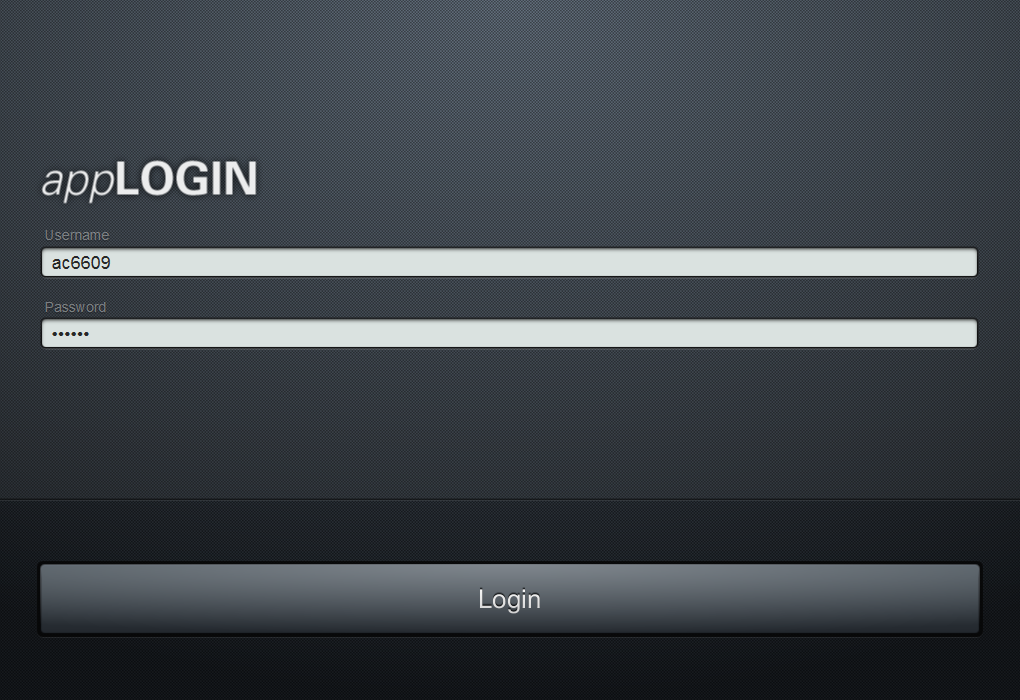
\includegraphics[scale=0.45]{login_screen}
\caption{The jSCAPE login screen.}
\label{fig:login_screen}
\end{figure}

For a student to use jSCAPE, they need to be in possession of login credentials, usually acquired by asking the appropriate teacher or lecturer. A connection to the jSCAPE system will be rejected if the entered login details are incorrect. Otherwise, the student can proceed to jSCAPE and access its features.

%show difficulty progression of exercises
\subsection{Practising programming}
\label{subsec:pratising-programming}
One of the main features of jSCAPE is the ability to practise programming through answering exercises. Selecting the Practice tab brings the student to a window where exercise categories, defined by the teacher, are displayed. These categories exist to separate exercises so that students can focus on practising one particular concept at a time. \newline

Figure \ref{fig:practice_overview} gives an overview of the Practice tab in jSCAPE. In this case, seven exercise categories have been defined by the teacher: Arrays, Loops, Syntax, Conditionals, Binary Trees, Strings and Objects. Order is irrelevant, students simply choose what type of exercise they want to practice.

\begin{figure}[H]
\centering
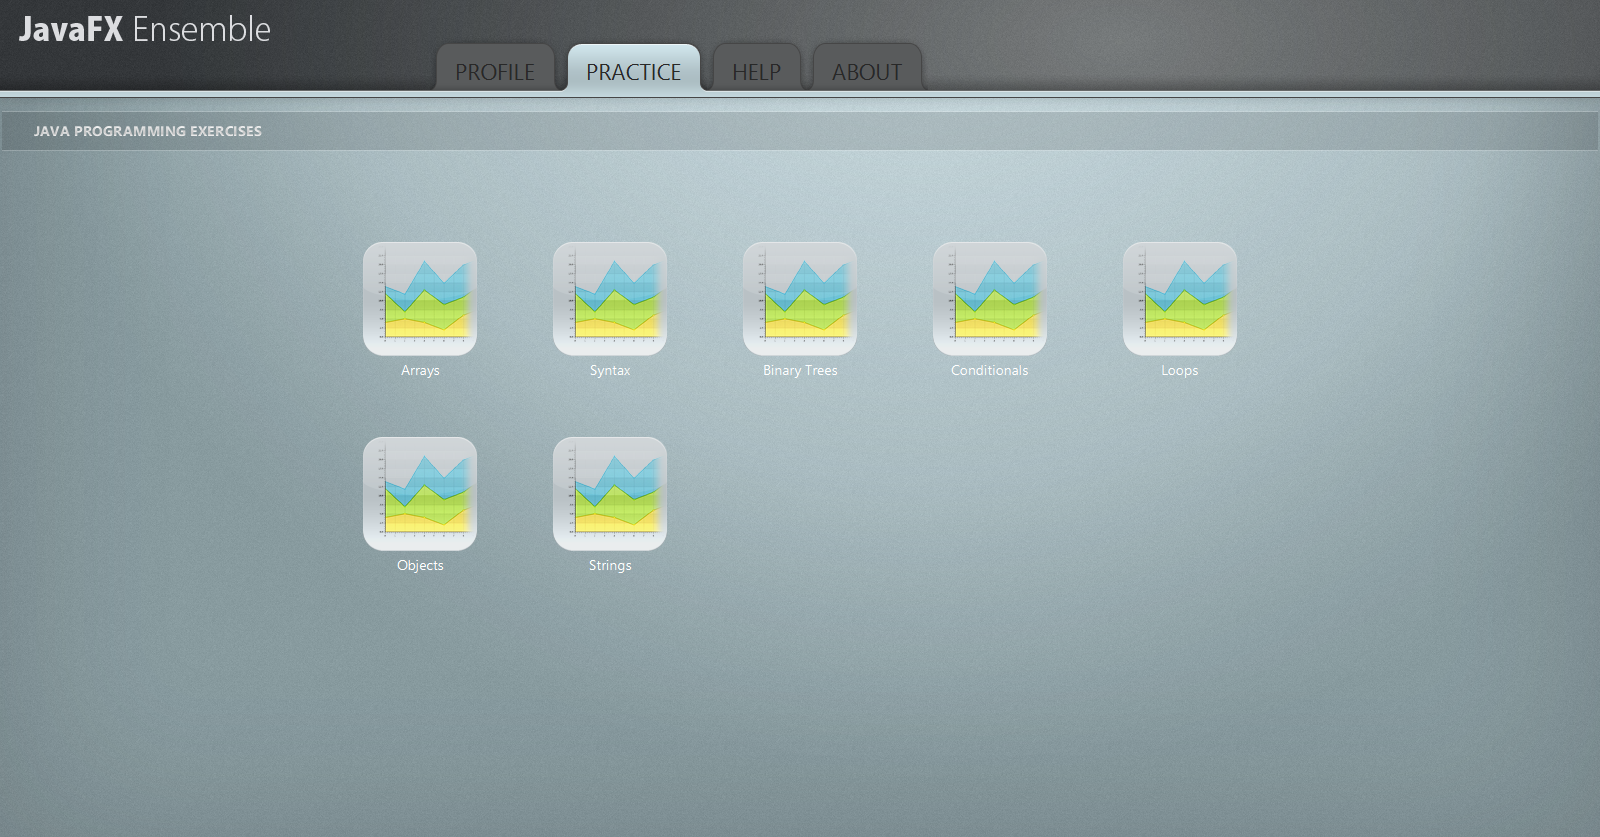
\includegraphics[width=\textwidth,height=\textheight,keepaspectratio]{practice_overview}
\caption{An overview of the Practice tab in jSCAPE.}
\label{fig:practice_overview}
\end{figure}

Clicking one of the exercise categories will bring the student to a new window, with an exercise and some helpful information about the chosen exercise category.
Figures \ref{fig:practice_binary_trees} and \ref{fig:practice_conditionals} give examples of what this exercise view can look like.\newline

In the case of the binary tree exercise (figure \ref{fig:practice_binary_trees}), exercise data, in the form of a binary tree, is displayed on the left of the window. On the right side of the window is the exercise itself, in this case it asks what should be printed if the binary tree is traversed using the in-order algorithm, and gives four options to choose from. It can be seen that the student has attempted to answer the exercise and has selected the wrong answer. This is indicated to the student in the form of ``wrong answer" in red. A correct answer would display ``correct answer" in green. Moreover the solution to the exercise is provided immediately after the student has answered it.

\newpage
\subsubsection{Example exercises}
\begin{figure}[H]
\centering
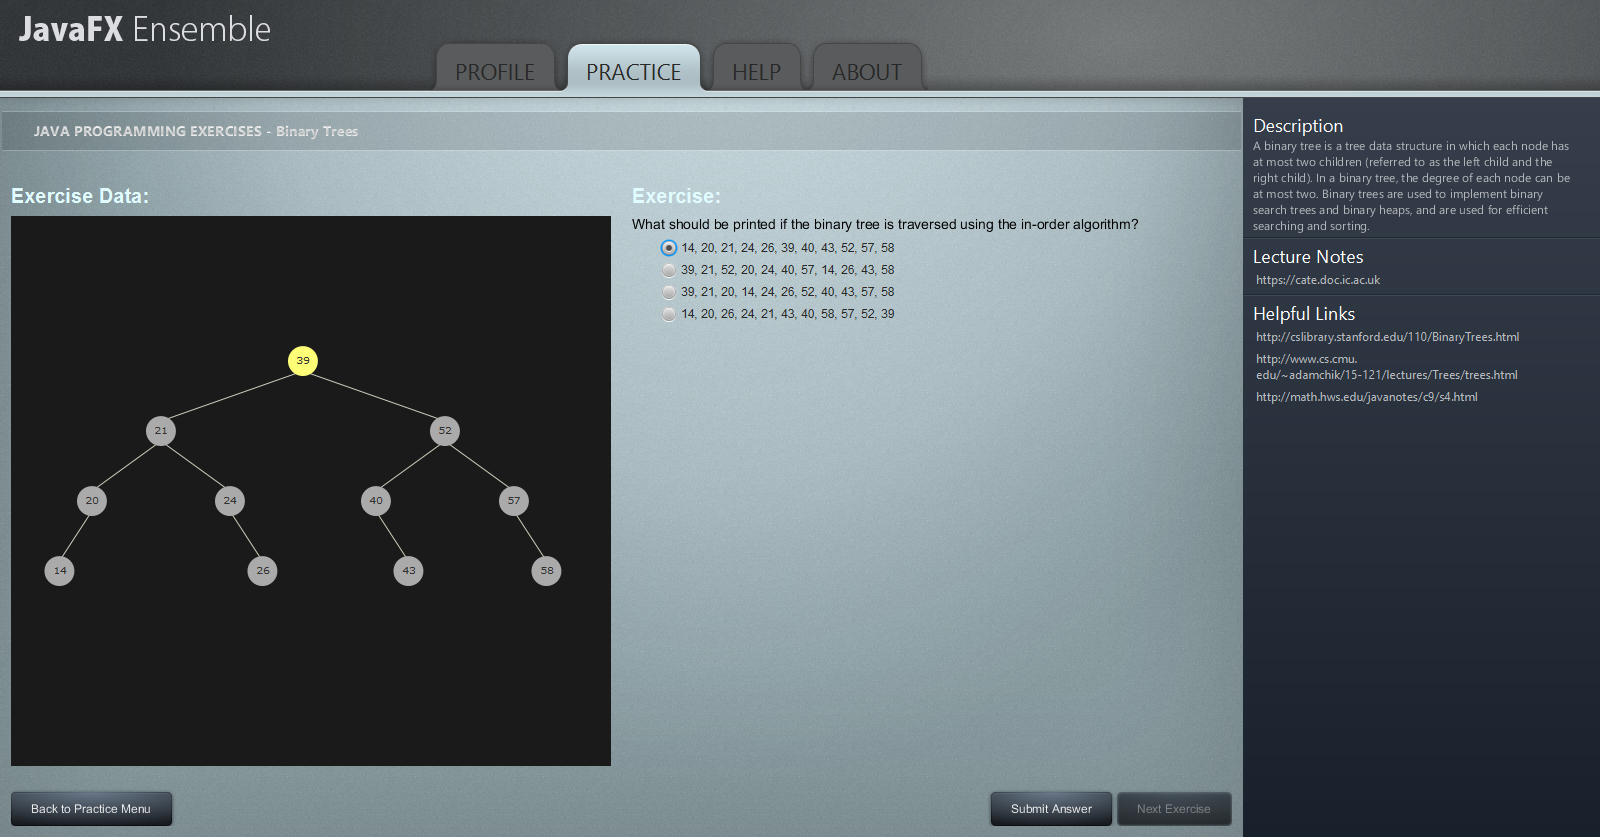
\includegraphics[width=\textwidth,height=\textheight,keepaspectratio]{practice_binary_trees}
\caption{The Practice tab view showing an exercise on binary trees.}
\label{fig:practice_binary_trees}
\end{figure}

\begin{figure}[H]
\centering
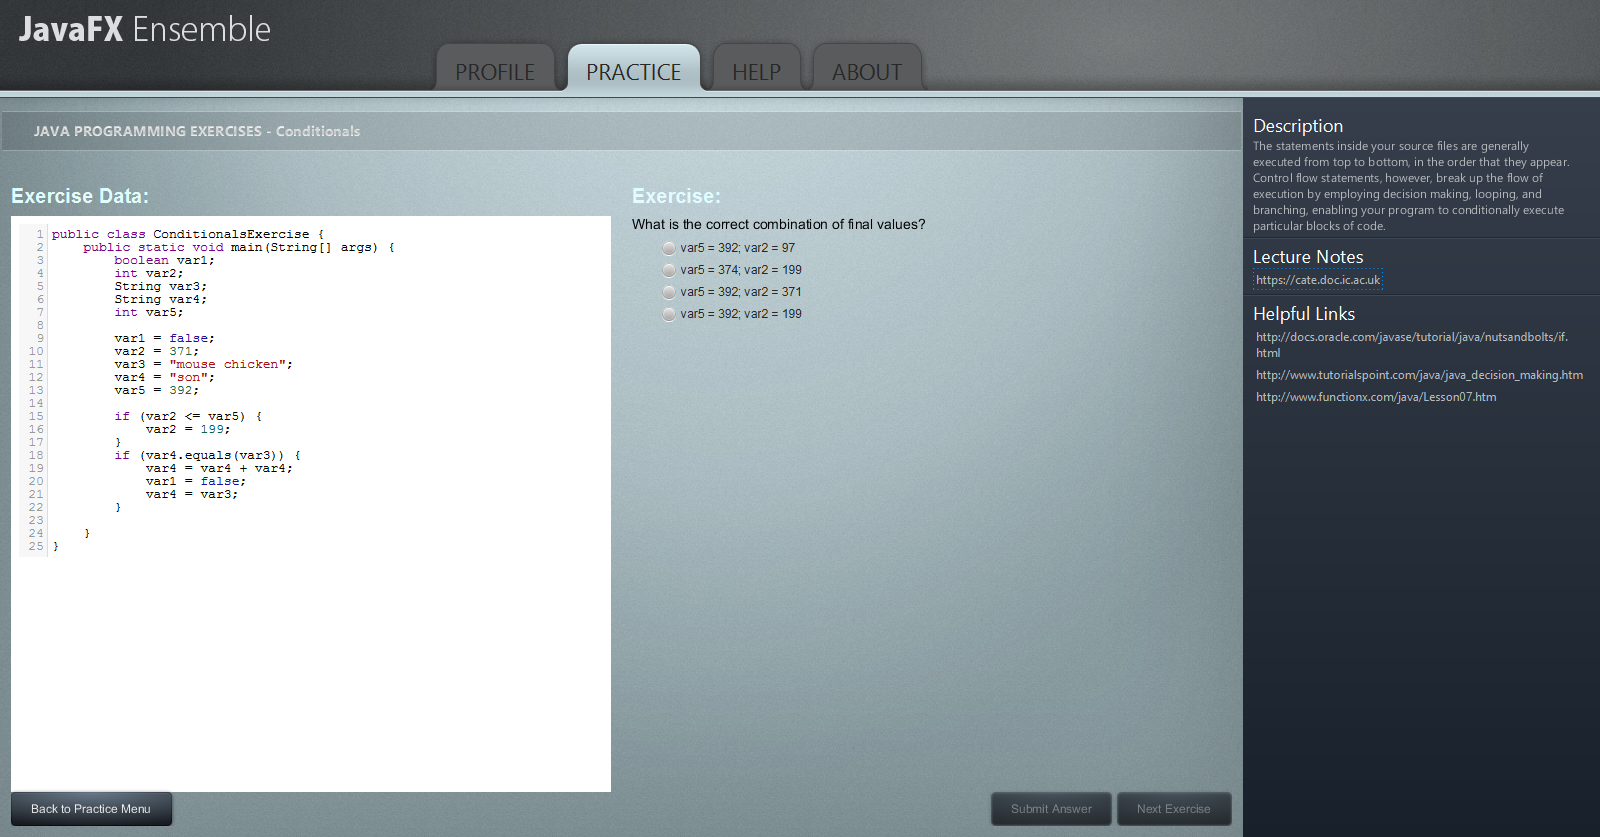
\includegraphics[width=\textwidth,height=\textheight,keepaspectratio]{practice_conditionals}
\caption{The Practice tab view showing an exercise on conditionals.}
\label{fig:practice_conditionals}
\end{figure}
\newpage

In the case of the exercise on conditionals (figure \ref{fig:practice_conditionals}), exercise data, in the form of a code fragment, is displayed on the left of the window. On the right side of the window is the exercise itself, in this case it asks the student to examine the code and to determine the final values of two variables, and provides again four options to choose from.

\begin{figure}[H]
\centering
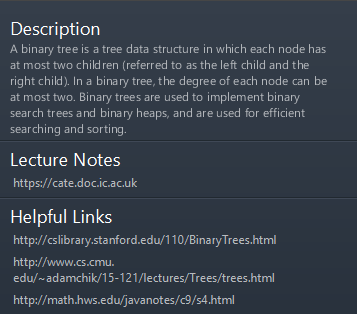
\includegraphics[scale=0.75]{practice_sidebar}
\caption{An example sidebar in the Practice tab.}
\label{fig:practice_sidebar}
\end{figure}

On the far right of every exercise, there is a dark blue sidebar which displays a description of the programming concept or construct being practised, links to university or course lecture notes and some other websites on the Internet if further help is needed. An example sidebar is shown in figure \ref{fig:practice_sidebar}, in this case the sidebar for the ``Binary Trees" exercise category.\newline

While answering exercises, students might notice how the difficulty of the exercises adapt to their performance. The system uses simple metrics to either increase or decrease the difficulty of exercises.\newline

For instance, for exercises in the Binary Tree category, the binary trees will increase in the number of nodes, or become very unbalanced. An example of this progression is shown in figure \ref{fig:binary_tree_progression}. \newline

For exercises in the Conditionals category, the number of \textsf{if} and \textsf{else} statements might increase or the exercise might ask for the final values of more variables.An example of this progression is shown in figure \ref{fig:conditionals_progression}.

\begin{figure}[H]
\centering
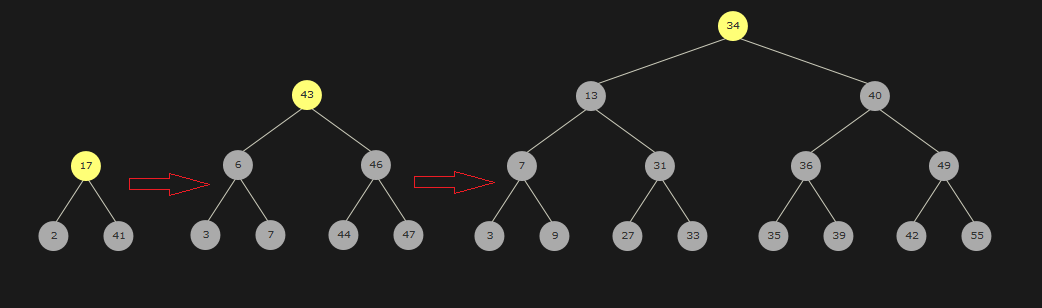
\includegraphics[width=\textwidth,height=\textheight,keepaspectratio]{binary_tree_progression}
\caption{Progression of binary tree exercises.}
\label{fig:binary_tree_progression}
\end{figure}

\begin{figure}[H]
\centering
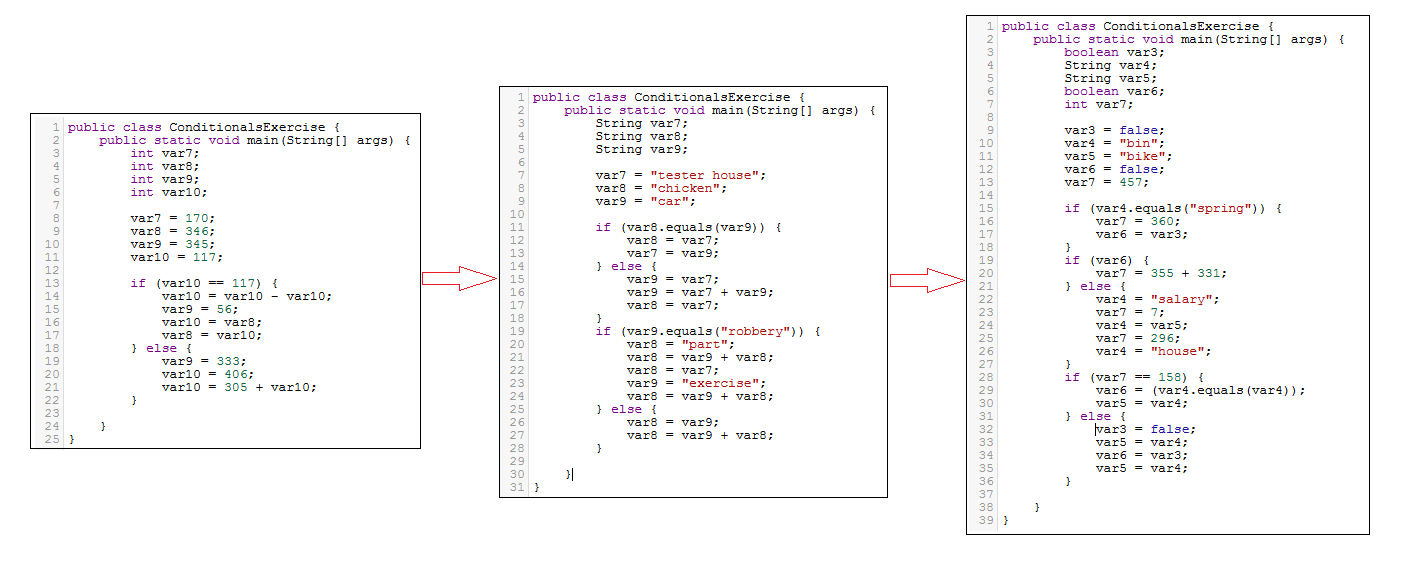
\includegraphics[width=\textwidth,height=\textheight,keepaspectratio]{conditionals_progression}
\caption{Progression of conditionals exercises.}
\label{fig:conditionals_progression}
\end{figure}

More details about how jSCAPE adapts the difficulty of exercises are given in section \ref{subsec:implementing-exercise-selection-algorithms} and section \ref{subsec:exercise-generation}.

\subsection{Tracking progress through statistical data}
\label{subsec:tracking-progress}
After a successful login the student lands on the Profile tab which presents information about the student, as well as statistical data on the student's performance and usage of the system.\newline

Figure \ref{fig:profile_screen_overview} shows the Profile tab after the student has logged in to the system. Profile information for the student is listed on the left hand side, in the light-blue rectangle. This information includes the student's first name, last name, user name, which class the student is in, the last time the student logged in, and the last time the student answered an exercise.

\begin{figure}[H]
\centering
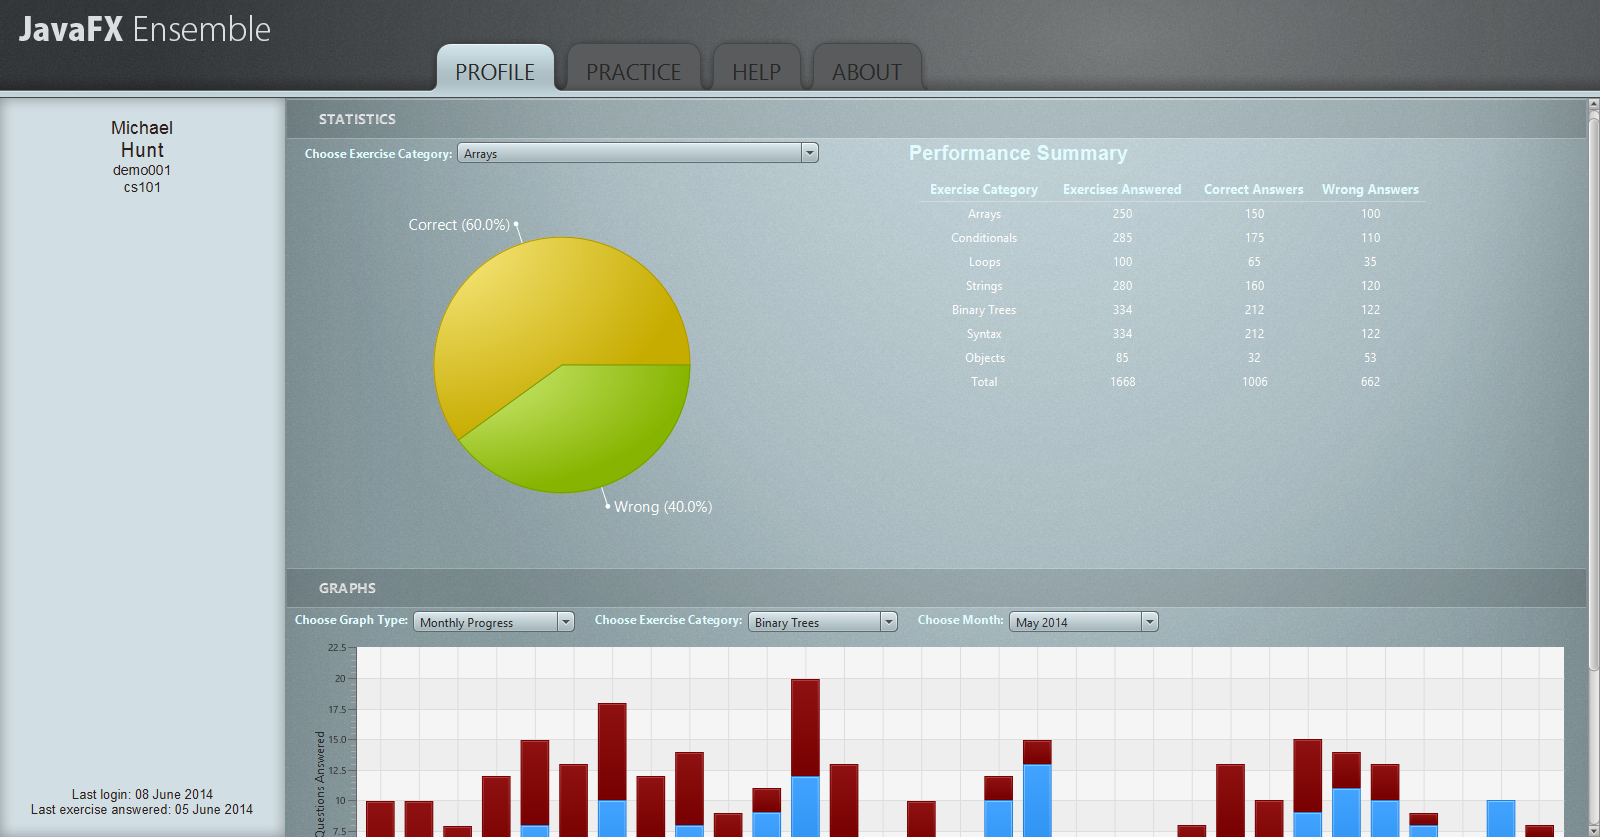
\includegraphics[width=\textwidth,height=\textheight,keepaspectratio]{profile_screen_overview}
\caption{An overview of the Profile tab in jSCAPE.}
\label{fig:profile_screen_overview}
\end{figure}

The main part of the Profile tab is split horizontally between statistical data in the form of pie charts and tables, and graphical data in the form of bar charts.

\begin{figure}[H]
\centering
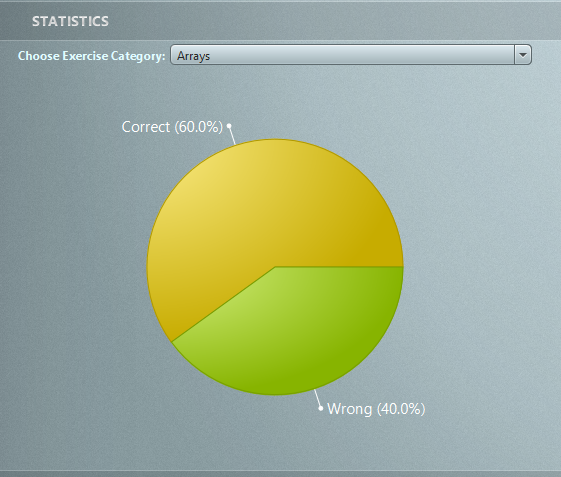
\includegraphics[scale=0.6]{pie_chart_stats}
\caption{Pie chart statistics for exercise category.}
\label{fig:pie_chart_stats1}
\end{figure}

Figure \ref{fig:pie_chart_stats1} shows the performance of the student in a particular exercise category, in this case ``Arrays". In the example, the student has gotten 60\% of array exercises correct and thus 40\% of them wrong. The student can view the performance pie chart for other exercise categories by changing the selected category in the combo box.

\begin{figure}[H]
\centering
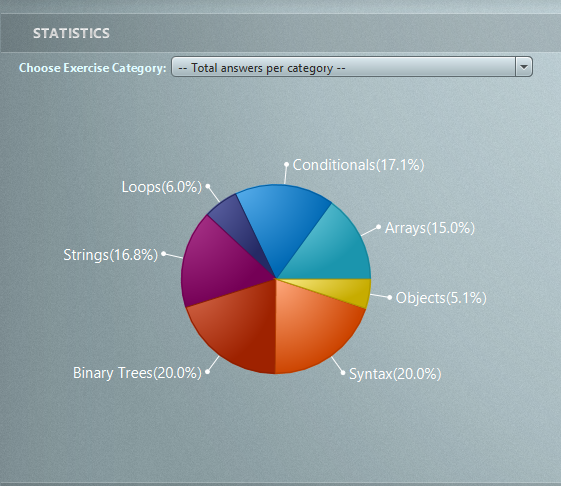
\includegraphics[scale=0.7]{pie_chart_stats2}
\caption{Pie chart statistics for distribution of answers.}
\label{fig:pie_chart_stats2}
\end{figure}

Another type of pie chart available in jSCAPE can be seen in figure \ref{fig:pie_chart_stats2}. This pie chart shows the distribution of answers per exercise category. This is a useful feature when a student is trying to get a balanced amount of practice in all exercise categories. \newline

Next, performance data is presented to the student in the performance summary table, shown in figure \ref{fig:performance_summary}. In this table, there is a row for every exercise category and a row for the total of each column. Each row contains the number of exercises answered, the number of correct answers and the number of wrong answers associated with a particular exercise category.

\begin{figure}[H]
\centering
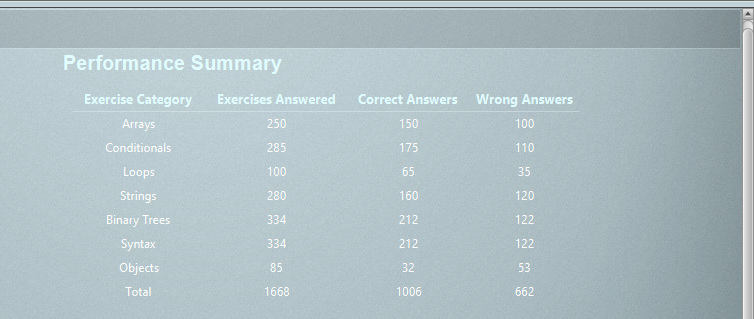
\includegraphics[width=\textwidth,height=\textheight,keepaspectratio]{performance_summary}
\caption{Performance summary table.}
\label{fig:performance_summary}
\end{figure}

In the lower half of the Profile tab there is the possibility to view performance data in the form of stacked bar charts.

\begin{figure}[H]
\centering
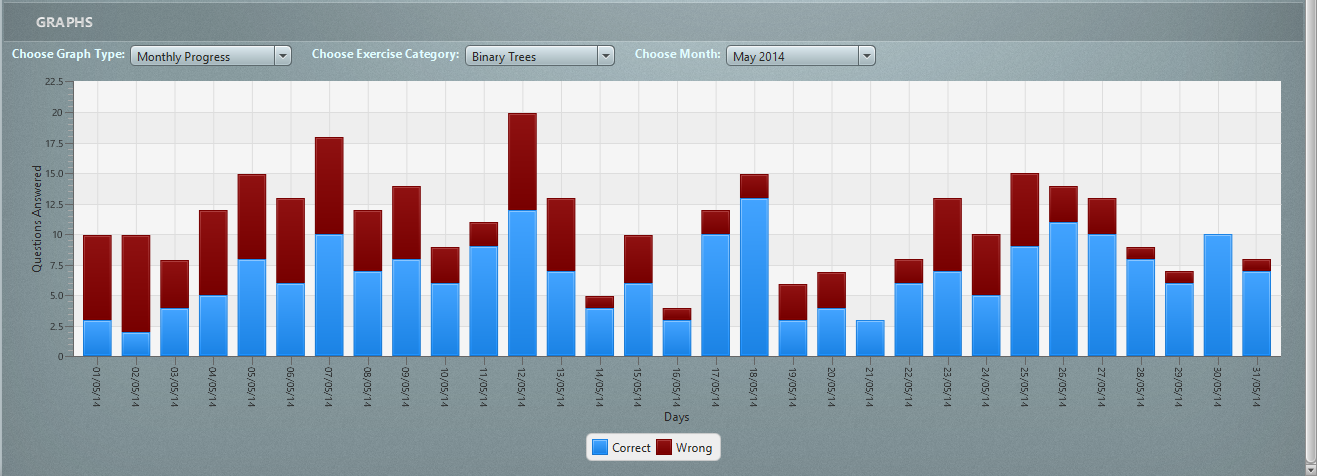
\includegraphics[width=\textwidth,height=\textheight,keepaspectratio]{monthly_progress}
\caption{Graph data of monthly progress.}
\label{fig:monthly_progress}
\end{figure}

Figure \ref{fig:monthly_progress} shows the monthly progress of a student for the month of May 2014 and for the exercise category ``Binary Trees". The number of correct answers (in blue) and wrong answers (in red) are graphed for each day where the student answered exercises. The student can view his monthly progress in other exercise categories and other months by manipulating the appropriate combo boxes. This historical data goes back to the first month in which the student answered an exercise.

\begin{figure}[H]
\centering
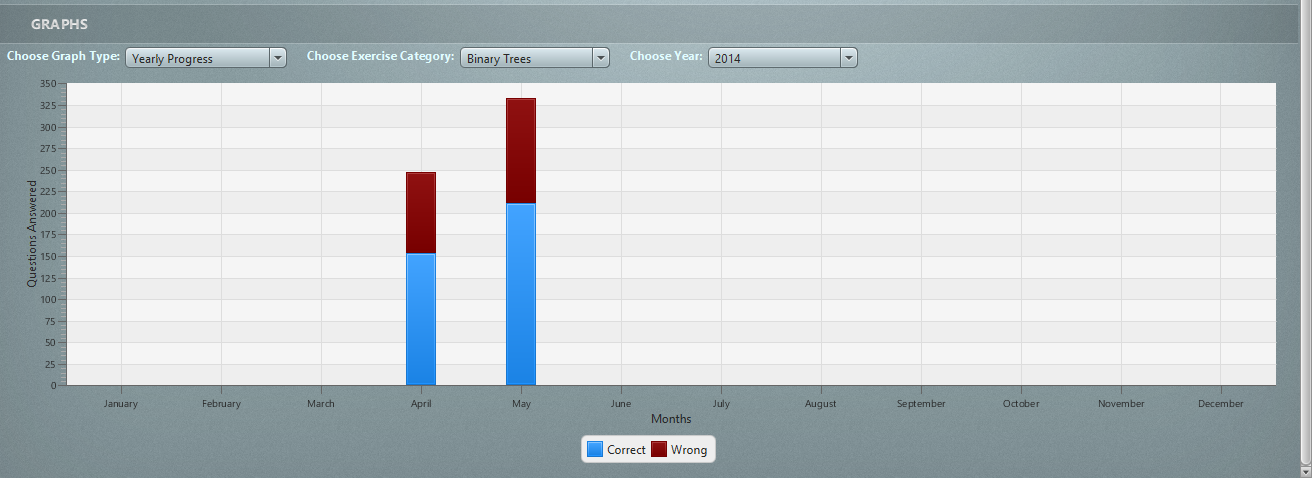
\includegraphics[width=\textwidth,height=\textheight,keepaspectratio]{yearly_progress}
\caption{Graph data of yearly progress.}
\label{fig:yearly_progress}
\end{figure}

Figure \ref{fig:yearly_progress} shows the yearly progress of a student in 2014 for the exercise category ``Binary Trees". For each month where the student answered exercises, a stacked bar can be found containing the total number of correct answers (in blue) and the total number of wrong answers (in red) for that particular year and exercise category. The student can view his yearly progress in other exercise categories and other years by manipulating the appropriate combo boxes. This historical data goes back to the year in which the student first started answering exercises.

\section{Teacher view}
The teacher's main access to the system is through the jSCAPE admin tool. Essentially it provides an interface to the database where all information about students, performance, exercise categories and exercises is stored. This tool was developed to allow teachers, not familiar with SQL, to still be able to retrieve useful data about students in a presentable way and to facilitate management of the exercise bank.

\subsection{Tracking student progress}
\begin{figure}[H]
\centering
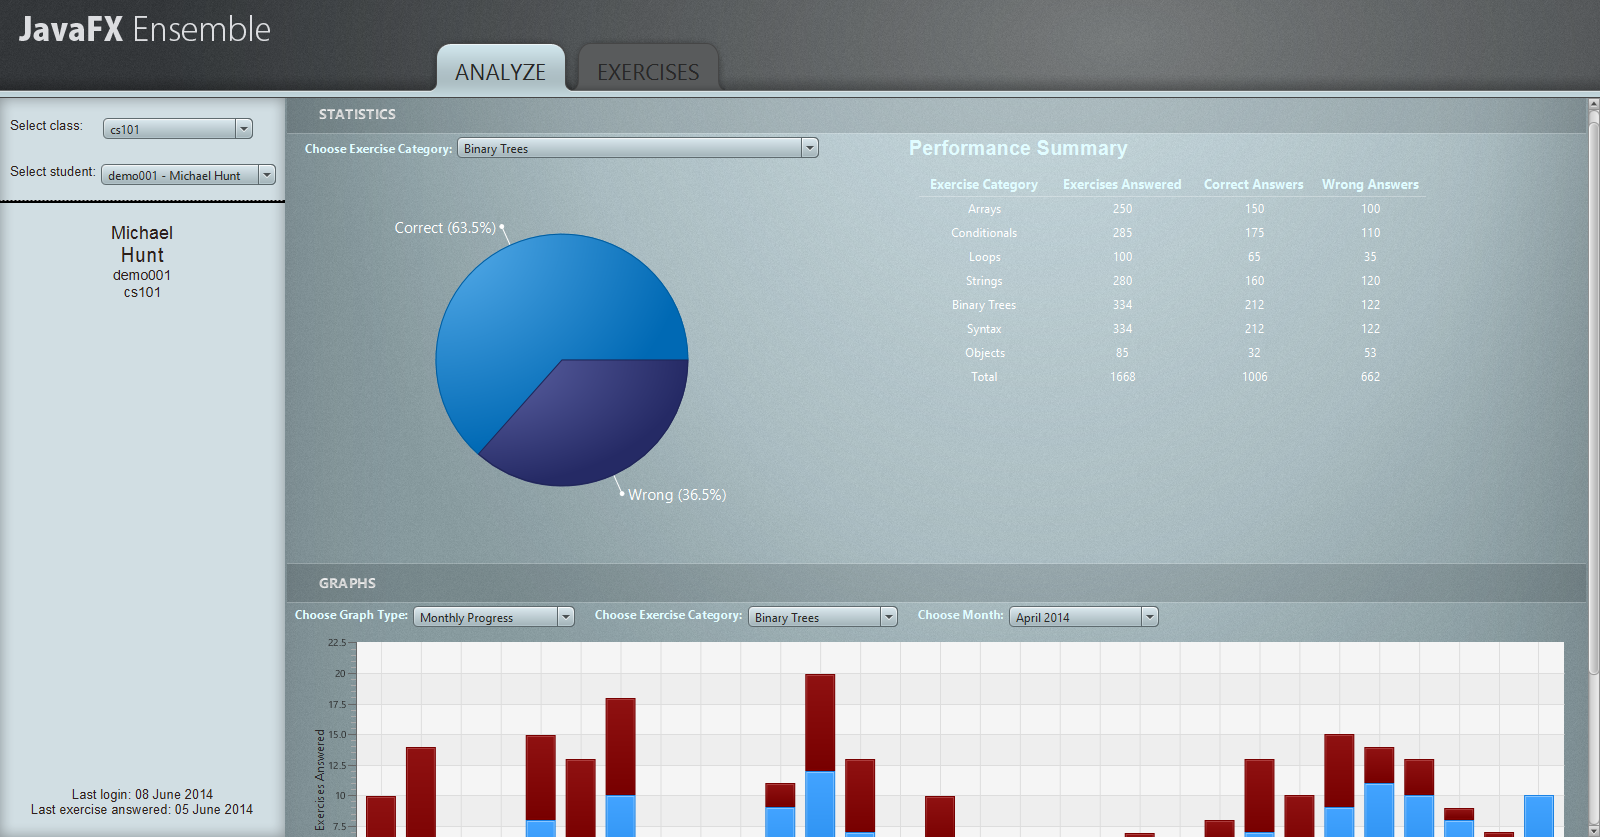
\includegraphics[width=\textwidth,height=\textheight,keepaspectratio]{analyze_overview}
\caption{An overview of the Analyze tab in the jSCAPE admin tool.}
\label{fig:analyze_overview}
\end{figure}

\begin{figure}[H]
\centering
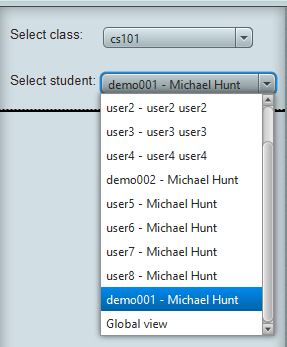
\includegraphics[scale=1]{analyze_select_student}
\caption{Selection possibilities in the Analyze tab.}
\label{fig:analyze_select_student}
\end{figure}

The jSCAPE admin tool provides teachers with the ability to track student progress and performance over time. Figure \ref{fig:analyze_overview} gives an overview of the Analyze tab, where statistical data about selected students can be displayed. The information displayed is identical to that displayed in the jSCAPE Profile tab (section \ref{subsec:tracking-progress}). On the left hand side of the window, the light blue box contains options to filter which data is displayed in the main window. A close up of the filter options is shown in figure \ref{fig:analyze_select_student}.\newline

The jSCAPE system includes support for multiple classes to allow for both the separation of students and the separation of exercises available to a class. A teacher can select a class to view statistics about those students taking the class. This will update the list of students in the combo box, allowing the teacher to focus his attention on the performance of one particular student. \newline

Selecting a student will show their profile information in the light blue window, along with the date of their last login, and the date of their last exercise answered. In addition, the pie charts, performance table and progress graphs will be updated to reflect the performance of the selected student. Finally, there is an option to obtain a global view of the class' performance by selecting the ``Global view" option. 

\begin{figure}[H]
\centering
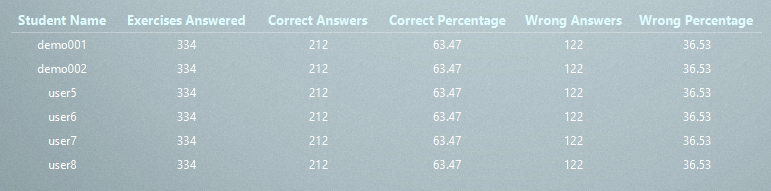
\includegraphics[width=\textwidth,height=\textheight,keepaspectratio]{global_view}
\caption{Global statistics view of a class.}
\label{fig:global_view}
\end{figure}

Figure \ref{fig:global_view} shows the table that is displayed after selecting the global view option. This table shows all the students who have answered exercises in a particular exercise category. In the example above, the data shown is for the ``Syntax" exercise category. The student user names are listed along with the number of exercises they have answered, and a detailed breakdown of the number of correct and wrong answers in terms of raw values and percentages. \newline

There is a combo box to select which exercise category to display, but this isn't shown in the picture to minimize the size of it. The global view feature is useful for teachers to identify which students may be facing difficulties. They can then select the student in the Analyze tab to get more detailed statistics and information about the student's progress.

\subsection{Managing the exercise bank}
A central feature of jSCAPE is providing programming exercises to students. The Exercise tab of the admin tool allows teachers to manage the exercise bank and perform functions such as adding new exercise categories, viewing existing exercises, adding new exercises manually and automatically generating more exercises.

\begin{figure}[H]
\centering
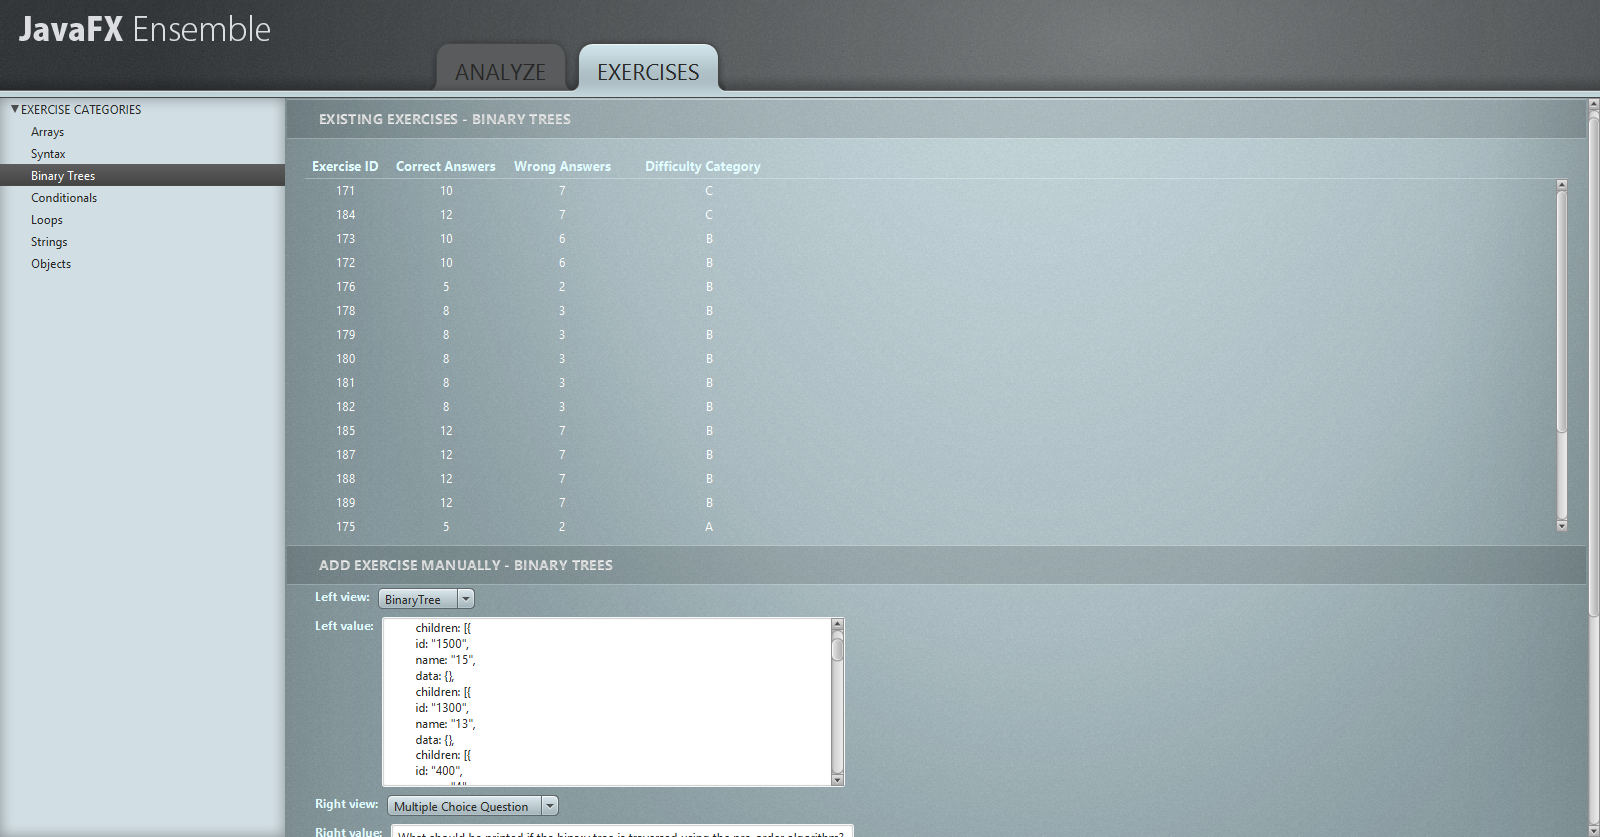
\includegraphics[width=\textwidth,height=\textheight,keepaspectratio]{exercises_admin_overview}
\caption{An overview of the exercise bank management tab.}
\label{fig:exercises_admin_overview}
\end{figure}

Figure \ref{fig:exercises_admin_overview} gives an overview of the Exercise tab. The light blue window on the left contains all existing exercise categories allowing the teacher to select which category they want to manage. In this case, the teacher has selected to view the exercise category ``Binary Trees", which displays the appropriate information in the main part of the tab, on the right.

\subsubsection{Managing exercise categories}
\begin{figure}[H]
\centering
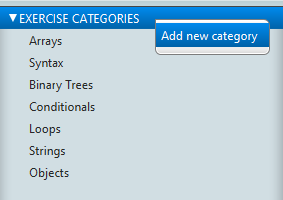
\includegraphics[scale=1]{add_exercise_category}
\caption{Adding a new exercise category.}
\label{fig:add_exercise_category}
\end{figure}

Figure \ref{fig:add_exercise_category} shows a close up of the light blue window. It lists all the existing exercise categories and selecting them will update the information displayed. Right-clicking on the root of the list opens up a context menu showing the possibility of adding a new exercise category. The definition of a new exercise category involves adding a description of the programming construct, some links to lecture notes and other helpful websites. These are of course optional. This information appears as part of the sidebar to an exercise as in figure \ref{fig:practice_sidebar}.\newline

There is also the possibility of choosing whether to make an exercise category visible or not to students. This is a useful feature if the class isn't ready to answer exercises of a particular category because the relevant material hasn't been taught yet, but the teacher still wants to prepare the exercises in advance to save time.
\subsubsection{Viewing existing exercises}
Once an exercise category has been selected from the list, several pieces of information are displayed.

\begin{figure}[H]
\centering
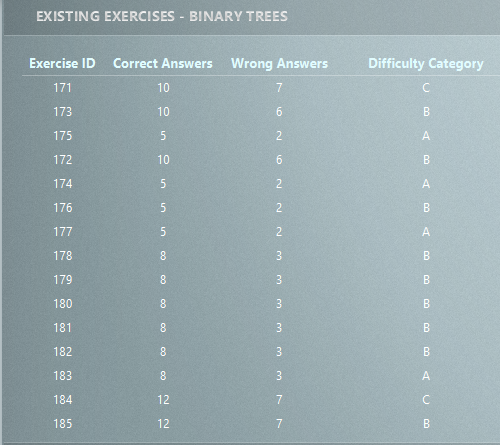
\includegraphics[scale=1]{existing_exercises}
\caption{Viewing information about existing exercises.}
\label{fig:existing_exercises}
\end{figure}

Figure \ref{fig:existing_exercises} shows one such piece of information. It is a table listing all the existing exercises of the selected exercise category which have been answered at least once by some student. The table lists some useful information about each exercise such as the exercise ID, the number of correct answers, the number of wrong answers and some information about difficulty.\newline

At the time of writing this report, the feature of double clicking a row to show the actual exercise description hasn't been implemented. We think that this would be a useful feature to have, enabling a teacher to view exactly which exercises students are getting right and wrong. However, a teacher competent with SQL and familiar with the jSCAPE system can still use the exercise ID as an index into the database table to retrieve further information about the exercise, including the actual exercise description.

\subsubsection{Automatically generating exercises}
\begin{figure}[H]
\centering
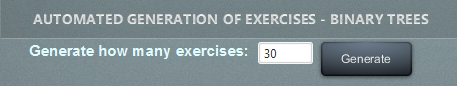
\includegraphics[scale=0.9]{automated_generation}
\caption{Automatically generating a number of new exercises for the Binary Tree exercise category.}
\label{fig:automated_generation}
\end{figure}

In jSCAPE teachers can automatically generate new exercises for a selected exercise category. The teacher inputs the number of exercises he wishes to generate, clicks the Generate button which will call the appropriate exercise generator, create the exercises and add them to the exercise bank. For more details about the implementation of the automated exercise generation process, refer to section \ref{subsec:exercise-generation}.

\subsubsection{Adding an exercise manually}
Although automatically generating exercises is a useful feature, it lacks the control offered by adding exercises manually. Indeed, the manual addition of exercises allows teachers to define exercises to target any identified student weaknesses. It also allows for more complex exercises which the automatic exercise generator wouldn't be able to produce. \newline

Figure \ref{fig:add_exercise_manually} shows an example of a teacher adding an exercise on binary trees to the exercise bank. Adding a new exercise manually consists in filling special tags which the jSCAPE system will recognize when trying to display the exercise to the student. These tags are:

\begin{itemize}
\item \textbf{Left view:} The name of the ``handler" that should be used in the left side of the exercise window. At the moment, two handlers exist. One is called BinaryTree for binary tree exercises, and another is called CodeEditor for exercises wishing to display pieces of code in the left view.
\item \textbf{Left value:} Code or text used by the handler to generate what appears in the left view. In the case of a binary tree exercise, it is the binary tree encoded in a JSON format. For code exercises, it is simply the code snippet to be displayed to the student.
\item \textbf{Right view:} The format of the exercise. Currently the system only supports multiple choice questions, but it would be quite easy to extend the system to support other types of exercises (section \ref{sec:future-work}).
\item \textbf{Right value:} The exercise description and the four possible choices.
\item \textbf{Solution:} The solution to the exercise.
\item \textbf{Difficulty:} Some attributes to indicate difficulty.
\end{itemize}

\begin{figure}[H]
\centering
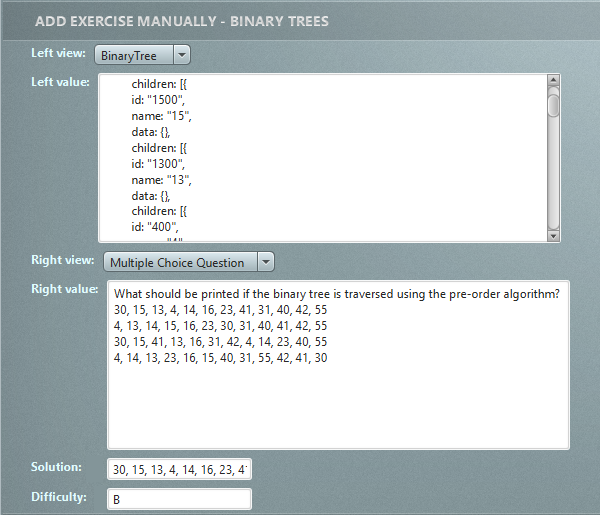
\includegraphics[width=\textwidth,height=\textheight,keepaspectratio]{add_exercise_manually}
\caption{Adding an exercise on binary trees manually.}
\label{fig:add_exercise_manually}
\end{figure}

For more details about the implementation of exercises and the various possibilities offered by the jSCAPE exercise format, refer to section \ref{sec:exercises-implementation}.\newline

Once these fields have all been filled in, the teacher can click the Add button and the exercise will be stored in the exercise bank and made available to students.

\section{Summary}
In this section we gave an overview of the two applications developed as part of this project: jSCAPE and the jSCAPE admin tool.\newline

We showed that jSCAPE provided an infrastructure for students to practice their understanding of programming concepts through exercises and to view their progress thanks to the extensive amount of statistical data collected by the system.\newline

In addition, we presented the jSCAPE admin tool, which allows teachers to define exercise categories, and add or generate exercises to create an environment suitable for student self-assessment. Finally, we showed features that enabled teachers to track student progress through the same statistical data displayed in the main application. \newline

In the following chapter, we talk more about the design of the system and various interesting implementation details and difficulties faced during the development of this project.

